\documentclass[11pt,ngerman]{article}
\usepackage{geometry}
\usepackage[T1]{fontenc}
\usepackage[utf8]{inputenc}
\usepackage{babel}
\usepackage{lmodern}%get scalable font
\usepackage{titling}
\usepackage{relsize}
\usepackage{biblatex}
\usepackage{hyperref}
\usepackage{paralist}
\usepackage[table, dvipsnames]{xcolor}
\usepackage{booktabs}
\usepackage{setspace}
\usepackage{float}
\usepackage{graphicx}
\usepackage{listings}

% Link colors
\hypersetup{
    colorlinks,
    linkcolor={blue},
    citecolor={red},
    urlcolor={blue}
}

% inline code macro
\definecolor{lightgray}{gray}{0.9}
\lstset{
    showstringspaces=false,
    basicstyle=\ttfamily,
    keywordstyle=\color{blue},
    commentstyle=\color[grey]{0.6},
    stringstyle=\color[RGB]{255,150,75}
}
\newcommand{\inlinecode}[2]{\colorbox{lightgray}{\lstinline[language=#1]$#2$}}

% Code block settings
\definecolor{codegreen}{rgb}{0,0.6,0}
\definecolor{codegray}{rgb}{0.5,0.5,0.5}
\definecolor{codepurple}{rgb}{0.58,0,0.82}
\definecolor{backcolour}{rgb}{0.95,0.95,0.92}

\lstdefinestyle{mystyle}{
    backgroundcolor=\color{backcolour},
    commentstyle=\color{codegreen},
    keywordstyle=\color{magenta},
    numberstyle=\tiny\color{codegray},
    stringstyle=\color{codepurple},
    basicstyle=\ttfamily\footnotesize,
    breakatwhitespace=false,
    breaklines=true,
    captionpos=b,
    keepspaces=true,
    numbers=left,
    numbersep=5pt,
    showspaces=false,
    showstringspaces=false,
    showtabs=false,
    tabsize=2
}
\lstset{style=mystyle}

% double quotes macro
% usage: \quotes{arg1}  => in text: "arg1"
\newcommand{\quotes}[1]{``#1''}

\geometry{a4paper, top=25mm, left=25mm, right=25mm, bottom=20mm,
    headsep=10mm, footskip=12mm}

\renewcommand{\arraystretch}{1.5}

\pretitle{\begin{center}\linespread{1.5}\huge}
    \posttitle{\par\end{center}\vspace{0.5em}}

\begin{document}

    \title{SWEN1\\Praktikum 05 Design Patterns\\
        \vspace{1cm}
        \small{ZHAW  School of Engineering\\Klasse: IT18tb\_zh}
        \vspace{1.5cm}
    }
    \author{
        Huber, Patrick\\
        \small{huberpa4@students.zhaw.ch}
        \vspace{1.5cm}
    }
   \date{\today}

    \maketitle
    \newpage

    \tableofcontents
    \listoffigures
    \lstlistoflistings
    \newpage

    \section{Praktikum Design Patterns}

    \subsection{Aufgabe 1 - Direkte Abhängigkeit vom Schalter zur Lampensteuerung vermeiden}
    \label{ssec:Aufg1}
    Um die direkt Abhängigkeit vom Schalter zur Lampensteuerung zu vermeiden, eignet sich das Composite Design Pattern. Es äre auch möglich das Abtract Factory Design Pattern anzuwenden, jedoch muss in diesem Beispiel noch von \inlinecode{Java}{JPanel} geerbt werden.

     \subsection{Aufgabe 2 - Abstraktionen für Lampe und Schalter}
    Wie in \autoref{ssec:Aufg1} bereits erwähnt, wurde für die Abstraktion - für Lampe und Schalter - das Composite Design Pattern gewählt. \newline Die Abstrakte Klasse \textbf{Lamp} (\autoref{lst:abstractClassLamp})  und die Abstrakte Klasse \textbf{Switch} (\autoref{lst:abstractClassSwitch})  sehen wie folgt aus:
     \vspace{.25cm}
    \lstinputlisting[language=Java,label={lst:abstractClassLamp}, caption=Abstrakte Klasse \textbf{Lamp}]{listings/Lamp.java}
    \vspace{.5cm}
    \lstinputlisting[language=Java, label={lst:abstractClassSwitch},caption=Abstrakte Klasse \textbf{Switch}]{listings/Switch.java}
    \vspace{.5cm}
    Das Klassendiagramm mit den Anpassungen sieht nun so aus:
    \begin{figure}[H]
        \centering
        \makebox[\textwidth][c]{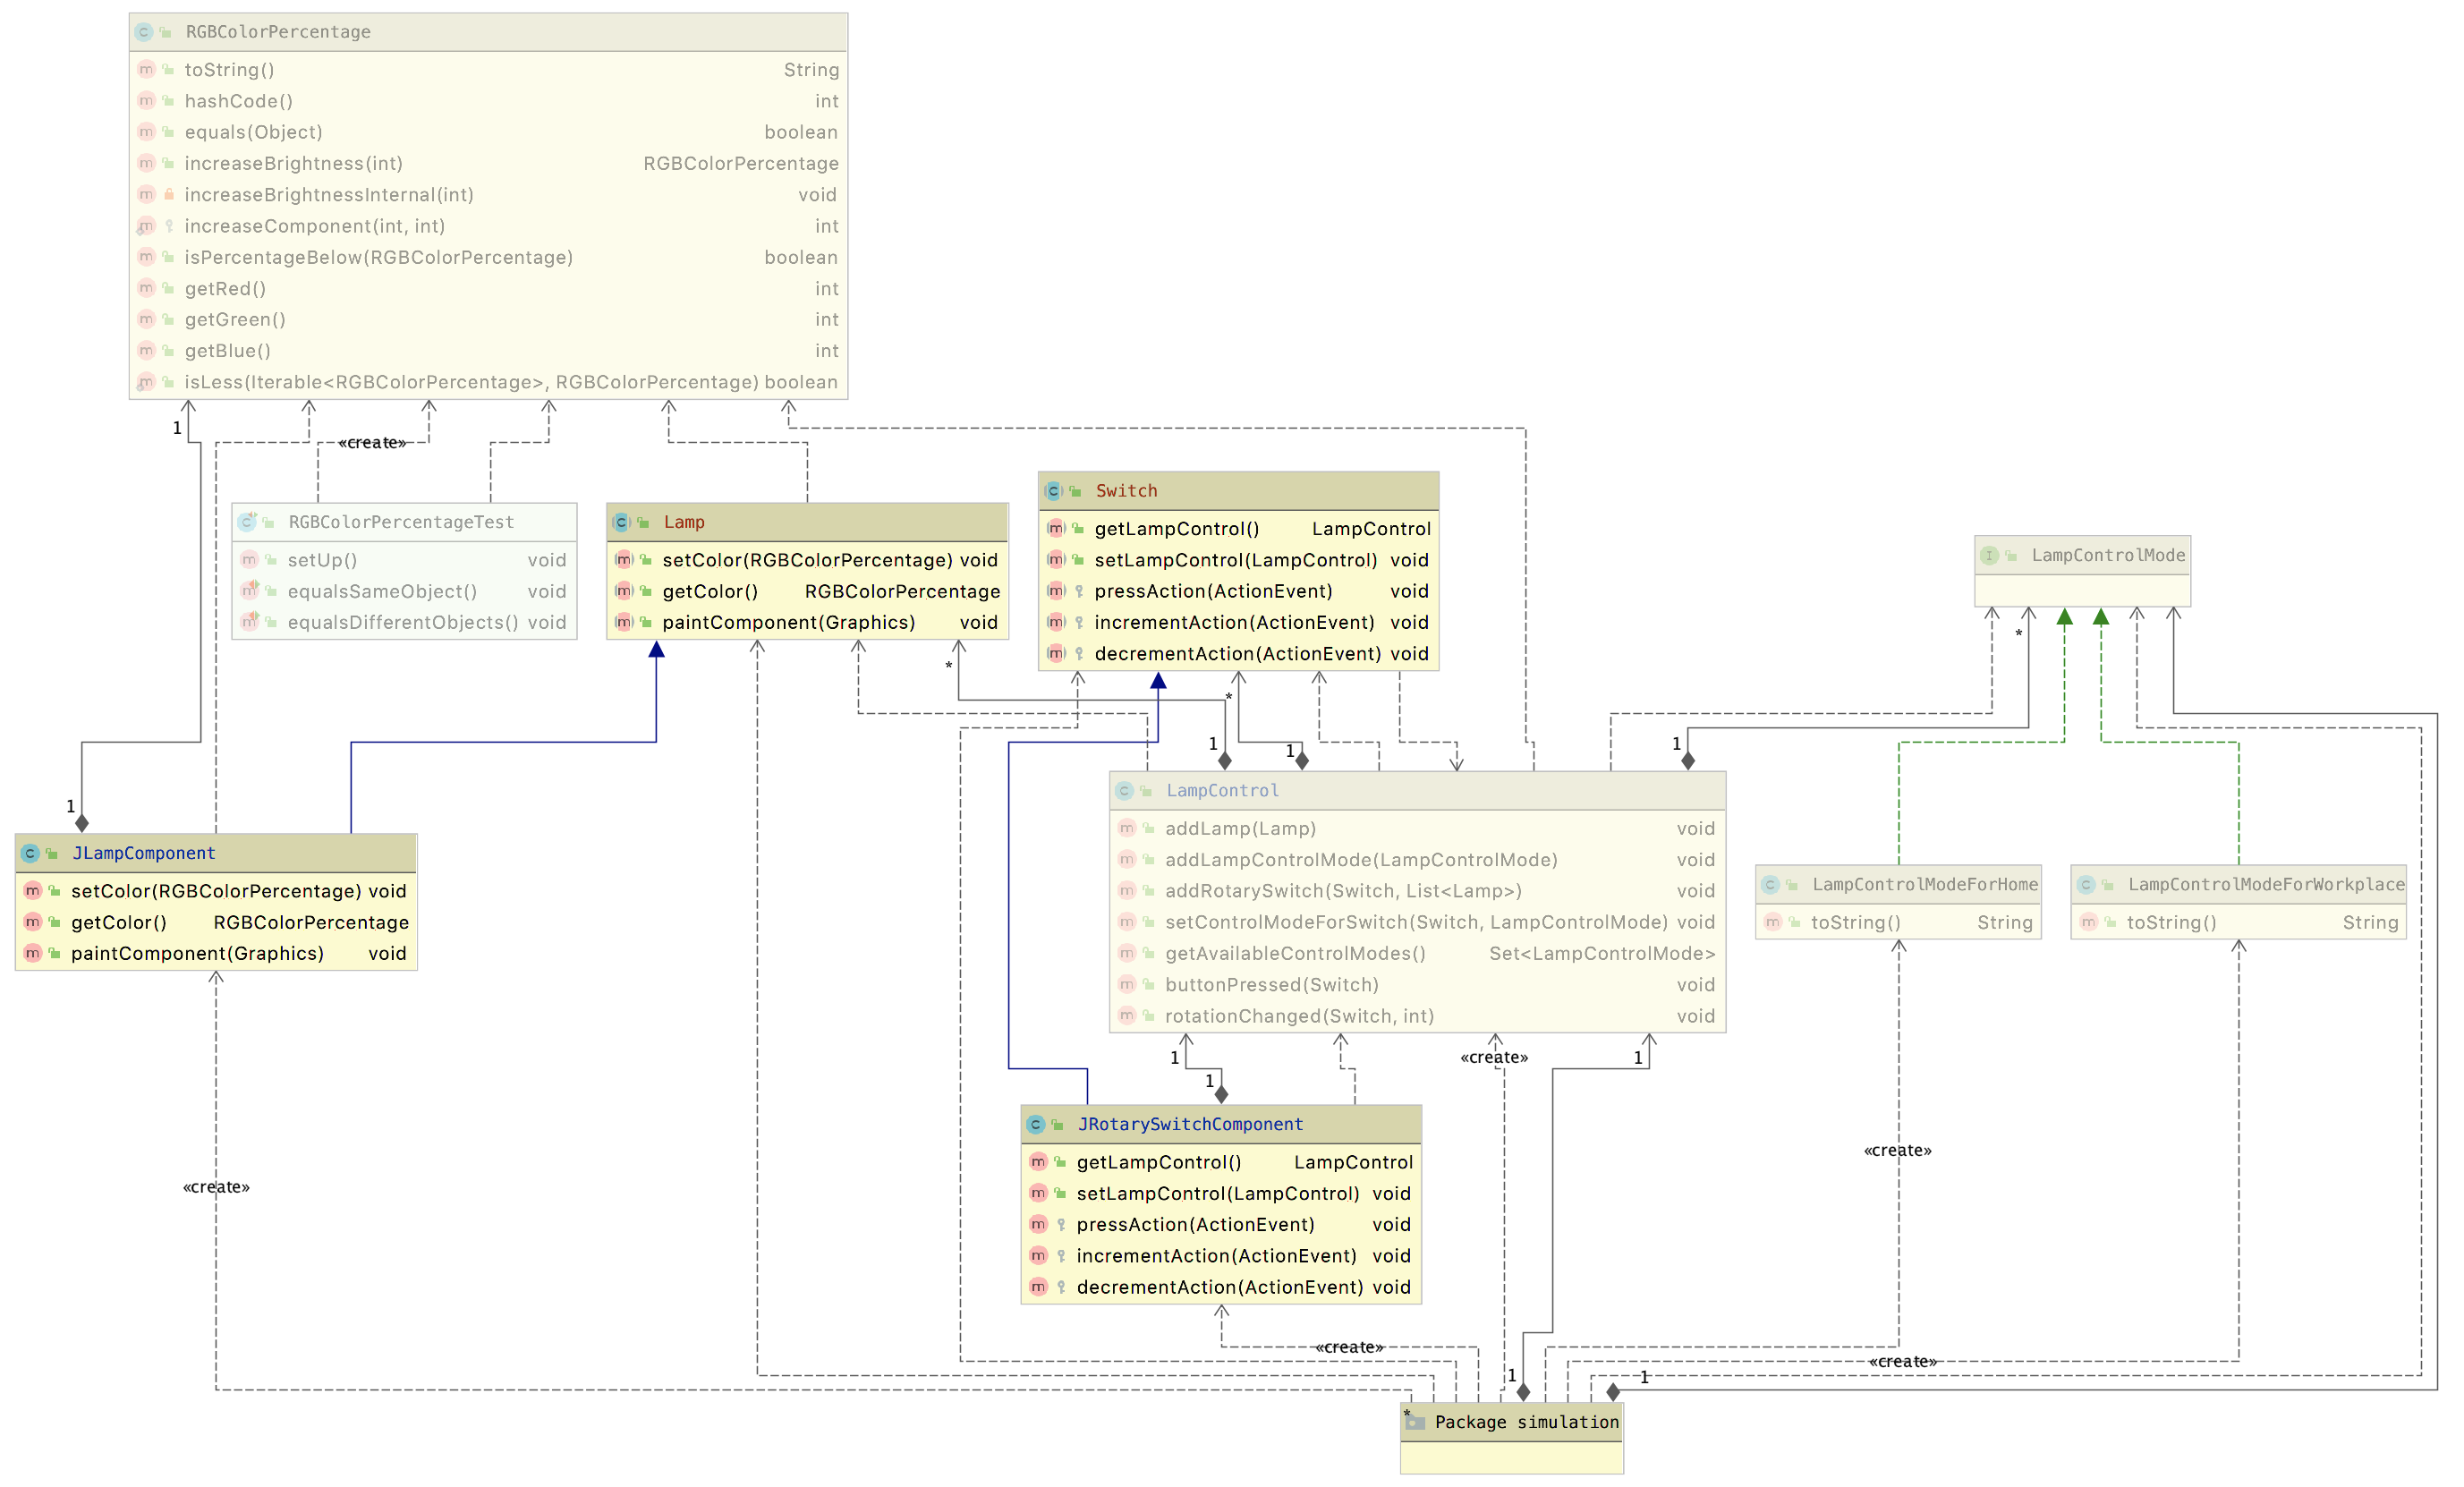
\includegraphics[width=1\textwidth]{figures/KlassenDiagramm_01.png}}
        \caption{UML Klassendiagramm  - Abstrakte Klassen \textbf{Switch} und \textbf{Lamp} wurden  implementiert.}
        \label{fig:ClassDiagram_Aufg2}
    \end{figure}


     \subsection{Aufgabe 3  \& 4 - Realisation Betriebsmodi}
     Jedem Schalter sind fix Lampen zugeordnet, die von ihm gesteuert werden. Pro Schalter kann einer der folgenden Betriebsmodi eingestellt werden:
     \begin{enumerate}
        \item \textbf{Arbeitsplatz}: Auf Druck des Schalters wird zwischen 0\% und 100\% umgeschaltet. Sollte der Wert dazwischen liegen, wird 0\% gesetzt. Eine Drehung des Schalters erhöht resp. reduziert die Helligkeit um 10\%.
        \item \textbf{Wohnung}: Auf Druck des Schalters wird zwischen 0\%, 45\%, 70\%, 85\% und 100\% umgeschaltet. Sollte der Wert dazwischen liegen, wird die nächst höhere Stufe gewählt, und wenn bereits 100\% erreicht ist, wird auf 0\% gesetzt. Eine Drehung des Schalters erhöht resp. reduziert die Helligkeit um 5\%.
    \end{enumerate}

    \noindent Die Betriebsmodi wurden mit dem Strategy Design Pattern  umgesetzt. Ein zusätzlicher Modus wurde ebenfalls implementiert.  Das Interface und die konkreten Modi sehen nun folgendermassen aus:
    \lstinputlisting[language=Java,label={lst:InterfaceLampControlMode}, caption=Interface \textbf{LampControlMode}]{listings/LampControlMode.java}
    \vspace{.5cm}
    \lstinputlisting[language=Java, label={lst:ClassLampControlModeForHome},caption=Klasse \textbf{LampControlModeForHome}]{listings/LampControlModeForHome.java}
    \vspace{.5cm}
    \lstinputlisting[language=Java, label={lst:ClassLampControlModeForStudy},caption=Klasse \textbf{LampControlModeForStudy}]{listings/LampControlModeForStudy.java}
    \vspace{.5cm}
    \lstinputlisting[language=Java, label={lst:ClassLampControlModeForWorkplace},caption=Klasse \textbf{LampControlModeForWorkplace}]{listings/LampControlModeForWorkplace.java}
    \vspace{.5cm}

    Das Klassendiagramm mit den Betriebsmodi-Anpassungen sieht nun so aus:
    \begin{figure}[H]
        \centering
        \makebox[\textwidth][c]{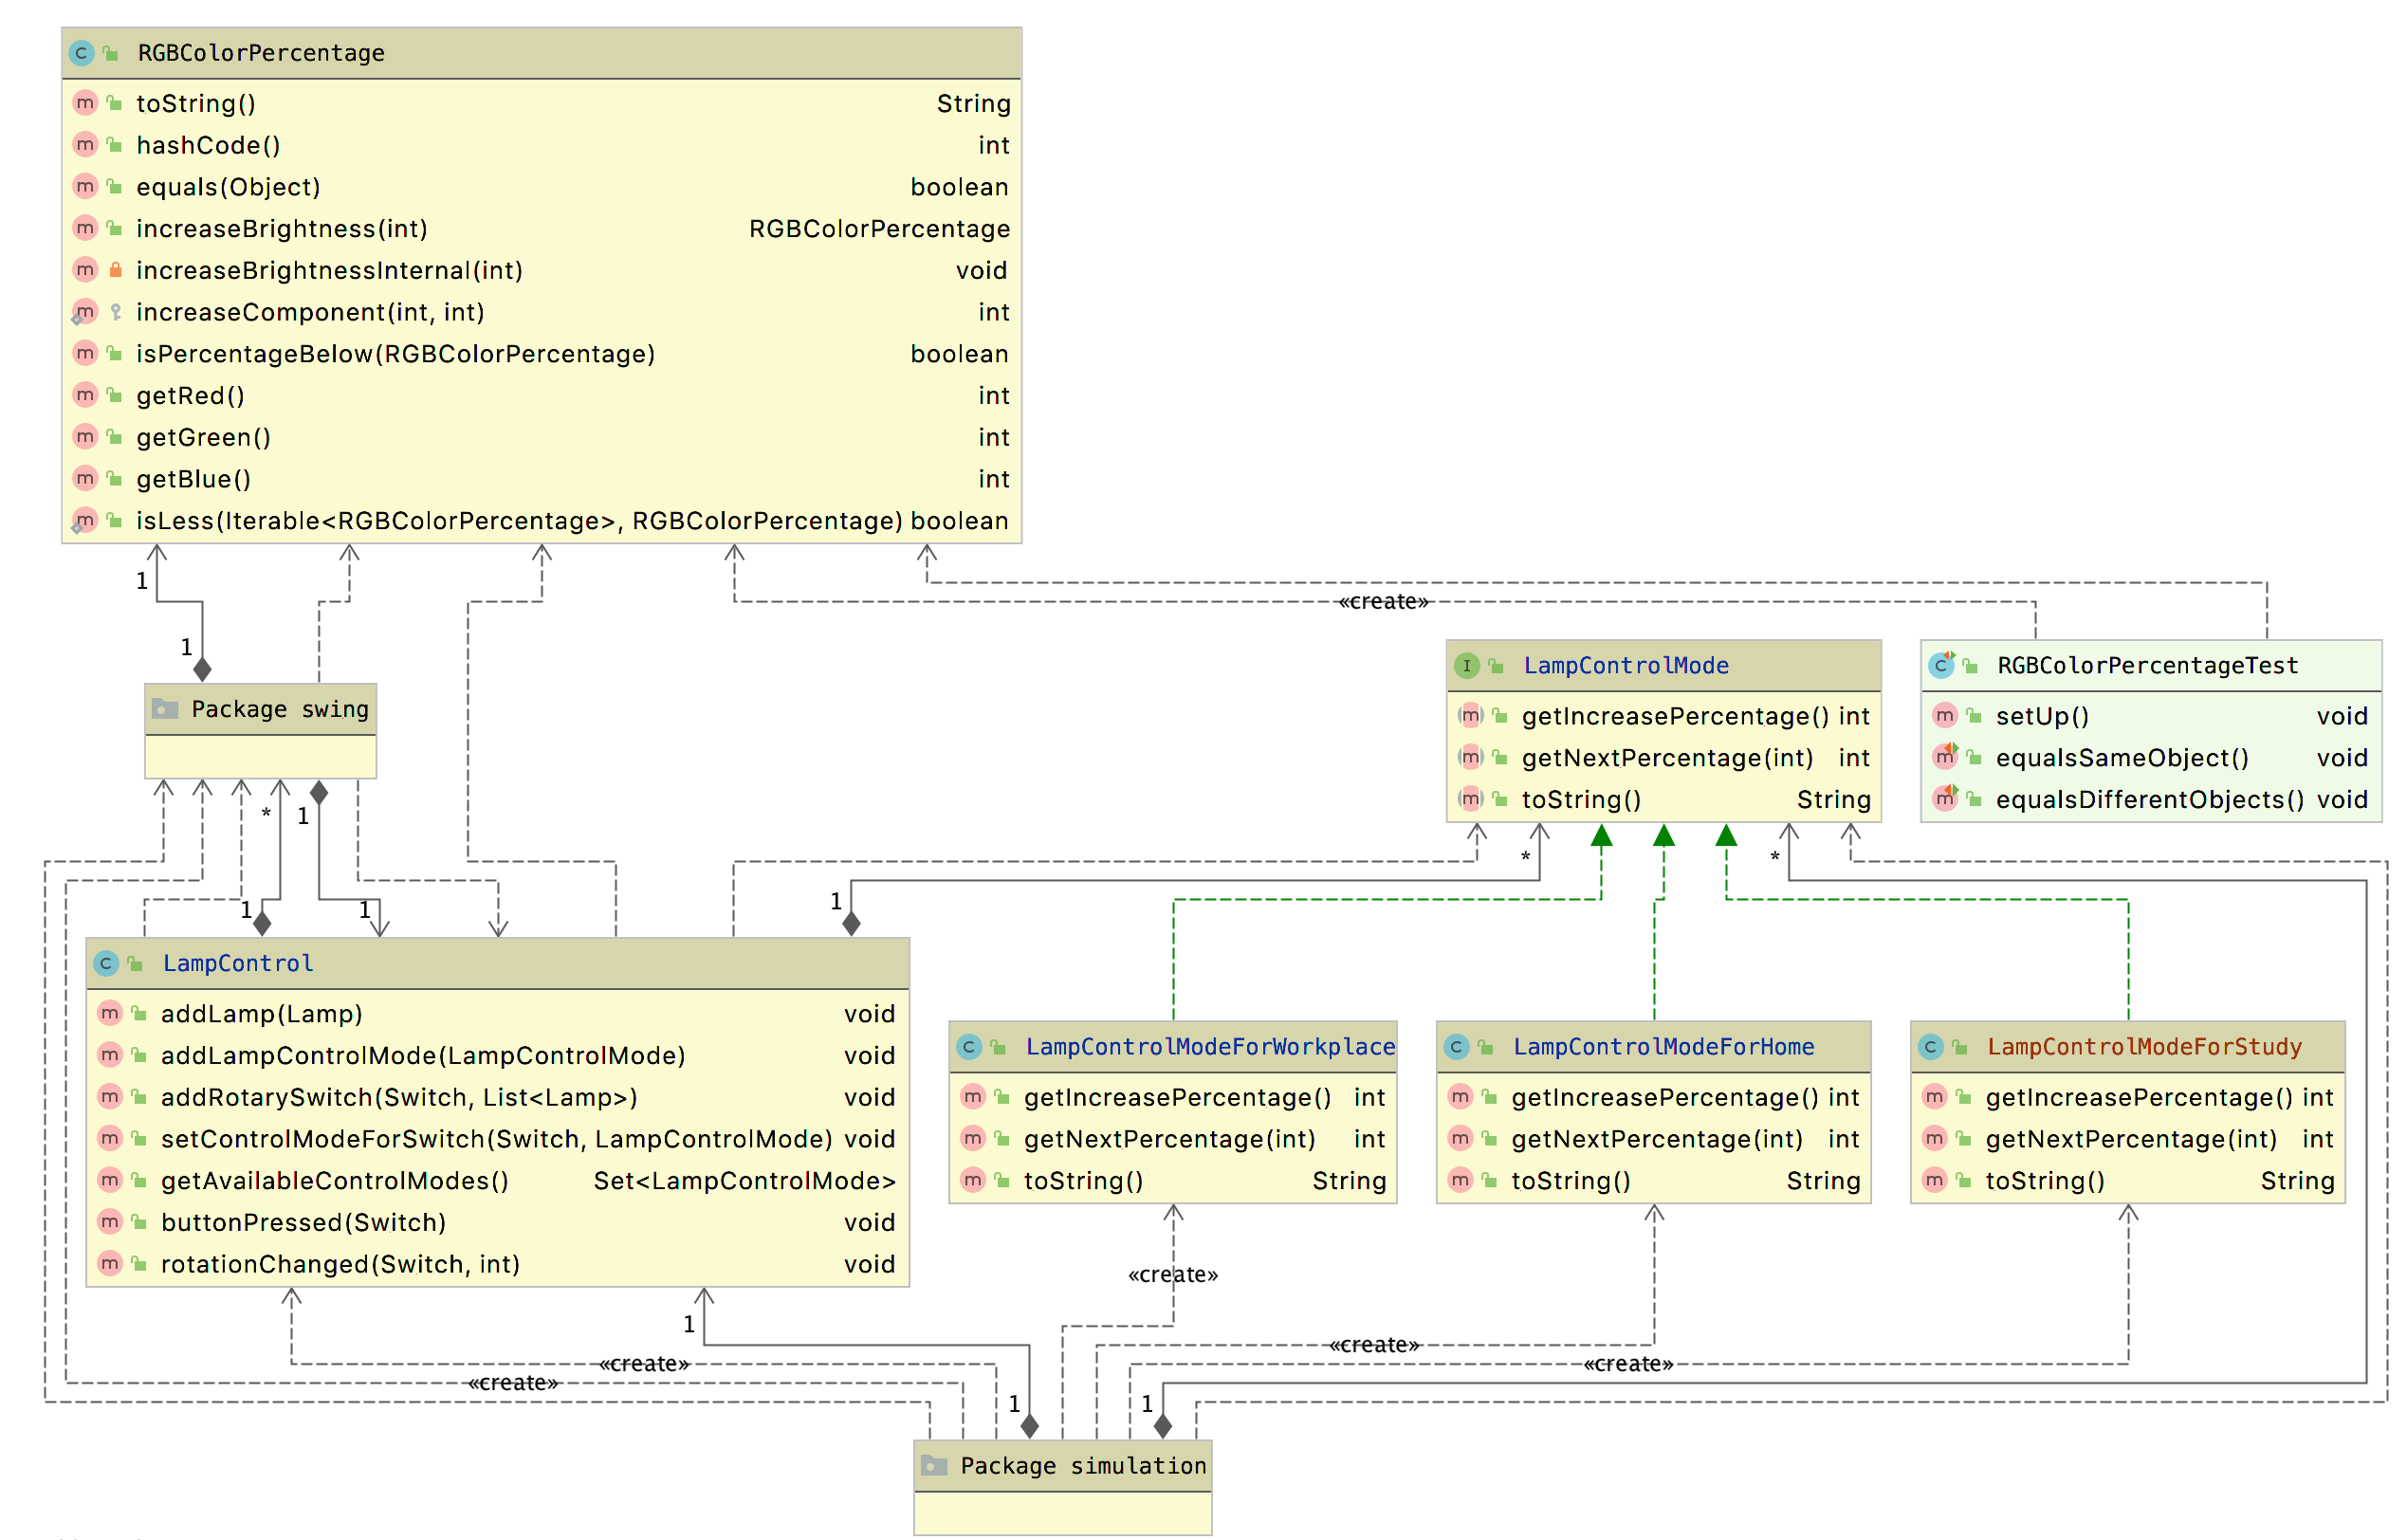
\includegraphics[width=1\textwidth]{figures/KlassenDiagramm_02.png}}
        \caption{UML Klassendiagramm  -  Betriebsmodi wurden implementiert}
        \label{fig:ClassDiagram_Aufg3}
    \end{figure}

    \subsection{Résumé}
    Diese \quotes{Applikation}  hat einige schwerwiegende Defizite. Ein Refactoring würde in diesem Umfang vermutlich mehr Zeit kosten als die Applikation neu zu designen und umzusetzen, zumal auch  richtige Testfälle fehlen, welche ebenfalls erst  geschrieben werden  müssten. Dazu kommt  noch \quotes{toter} Code, der  nicht mehr in Gebrauch ist. Die gesamte Applikation hat, meiner Meinung nach, eine geringe Kohäsion und eine hohe Kopplung, ist eher prozedural als objekt-orientiert umgesetzt worden. Ein weiteres Problem ist die Kopplung von der Darstellung mit Teilen der Applikationslogik. Leider fehlt mir die Zeit für eine neue Umsetzung, da wir durch PSIT3 Abgabe enorm gefordert sind.Aus diesem Grund habe ich auch keine weiteren Testfälle geschrieben.

    \subsection{Java Code}
    \label{ssec:Codeausschnitte}
    Alle relevanten Code-Dateien sind hier aufgeführt. \newline
    \textit{Hinweis}: Der ganze Quelltext kann unter folgendem Link angesehen werden: \\ \url{https://github.zhaw.ch/huberpa4/SWEN1/tree/master/Praktikum_Patterns-HS20}

\subsubsection{Datei RGBColorPercentageTest.java}
\lstinputlisting[language=Java, caption=Code RGBColorPercentageTest.java]{listings/RGBColorPercentageTest.java}
\vspace{.5cm}

\subsubsection{Datei LampControlModeForStudy.java}
\lstinputlisting[language=Java, caption=Code LampControlModeForStudy.java]{listings/LampControlModeForStudy.java}
\vspace{.5cm}

\subsubsection{Datei LampControlModeForWorkplace.java}
\lstinputlisting[language=Java, caption=Code LampControlModeForWorkplace.java]{listings/LampControlModeForWorkplace.java}
\vspace{.5cm}

\subsubsection{Datei LampControlModeForHome.java}
\lstinputlisting[language=Java, caption=Code LampControlModeForHome.java]{listings/LampControlModeForHome.java}
\vspace{.5cm}

\subsubsection{Datei Lamp.java}
\lstinputlisting[language=Java, caption=Code Lamp.java]{listings/Lamp.java}
\vspace{.5cm}

\subsubsection{Datei LampControlMode.java}
\lstinputlisting[language=Java, caption=Code LampControlMode.java]{listings/LampControlMode.java}
\vspace{.5cm}

\subsubsection{Datei Switch.java}
\lstinputlisting[language=Java, caption=Code Switch.java]{listings/Switch.java}
\vspace{.5cm}

\subsubsection{Datei JLampComponent.java}
\lstinputlisting[language=Java, caption=Code JLampComponent.java]{listings/JLampComponent.java}
\vspace{.5cm}

\subsubsection{Datei JRotarySwitchComponent.java}
\lstinputlisting[language=Java, caption=Code JRotarySwitchComponent.java]{listings/JRotarySwitchComponent.java}
\vspace{.5cm}

\subsubsection{Datei SwitchFrame.java}
\lstinputlisting[language=Java, caption=Code SwitchFrame.java]{listings/SwitchFrame.java}
\vspace{.5cm}

\subsubsection{Datei Lamp.java}
\lstinputlisting[language=Java, caption=Code Lamp.java]{listings/Lamp.java}
\vspace{.5cm}

\subsubsection{Datei Switch.java}
\lstinputlisting[language=Java, caption=Code Switch.java]{listings/Switch.java}
\vspace{.5cm}

\subsubsection{Datei LightingAppMainFrame.java}
\lstinputlisting[language=Java, caption=Code LightingAppMainFrame.java]{listings/LightingAppMainFrame.java}
\vspace{.5cm}

\subsubsection{Datei LampControlModeForStudy.java}
\lstinputlisting[language=Java, caption=Code LampControlModeForStudy.java]{listings/LampControlModeForStudy.java}
\vspace{.5cm}

\subsubsection{Datei RGBColorPercentage.java}
\lstinputlisting[language=Java, caption=Code RGBColorPercentage.java]{listings/RGBColorPercentage.java}
\vspace{.5cm}

\subsubsection{Datei LampControlModeForWorkplace.java}
\lstinputlisting[language=Java, caption=Code LampControlModeForWorkplace.java]{listings/LampControlModeForWorkplace.java}
\vspace{.5cm}

\subsubsection{Datei LampControl.java}
\lstinputlisting[language=Java, caption=Code LampControl.java]{listings/LampControl.java}
\vspace{.5cm}

\subsubsection{Datei LampControlModeForHome.java}
\lstinputlisting[language=Java, caption=Code LampControlModeForHome.java]{listings/LampControlModeForHome.java}
\vspace{.5cm}

\subsubsection{Datei LampControlMode.java}
\lstinputlisting[language=Java, caption=Code LampControlMode.java]{listings/LampControlMode.java}
\vspace{.5cm}

\end{document}

